\newpage
\subsection{Detachable module}
\label{subsec:detachable_module} 

In this last subsection of the electronics will be described the need and the design of the detachable module.

\subsubsection{Functionality}
\label{subsubsec:detachable_module/functionality} 

To clarify the need of a detachable module, the plush toy was required to be washable. 

\medskip At the current stage of the project, to avoid the complexity of trying to get a perfectly waterproof mechanical box, in which all the hard electronics will be embedded (refer to section \ref{sec:me}), the textile wires needed to be detachable from the main PCB. To this aim, a detachable module has been designed, to connect the sewed textile wires with the main PCB, in contact with its pins with the holes of the module. 

\medskip In this manner, the pins of the main PCB can be temporarily connected with the LEDs and the capacitive touch sensors. 

\medskip Despite the notation of "detachable" that can have several connotations, the module would be fixed on the plush toy and eventually washed with it. Before being able to wash the plush toy, the user shall detach beforehand the mechanical box from the plush toy and thus from this "detachable module".

\subsubsection{Schematic}
\label{subsubsec:detachable_module/schematic} 

The very simplistic schematic of the detachable PCB is shown figure \ref{fig:detachable_module_schematic}.

\begin{figure}[H]
    \centering
    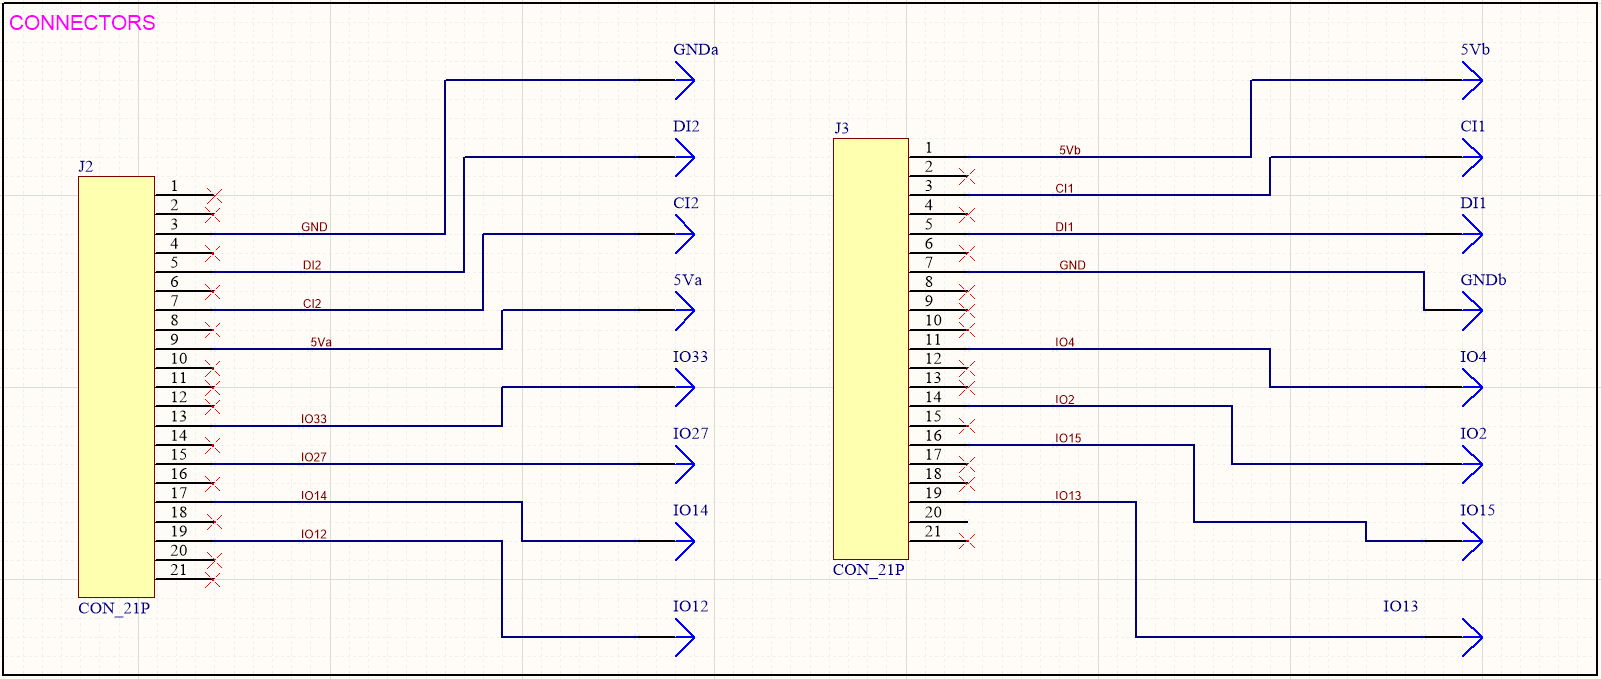
\includegraphics[width=0.9\textwidth]{images/EE_DetachableModuleSchematic.PNG}
    \caption{Detachable module schematic}
    \label{fig:detachable_module_schematic}
\end{figure}

The only components of this schematic are :

\begin{itemize}
    \item the pads (indicated with arrows), to be connected with the textile wires coming from the LEDs and the capacitive touch sensors and 
    \item the 21 mounting holes (indicated with rectangles), to be connected on the two 21-header-pins of the main PCB.
\end{itemize}


\subsubsection{Detachable module design}
\label{subsubsec:detachable_module/design} 

Figure \ref{fig:detachable_module_2D} illustrates the 2D view of the detachable PCB, 55.61 mm long and 42.40 mm wide.

\begin{figure}[H]
    \centering
    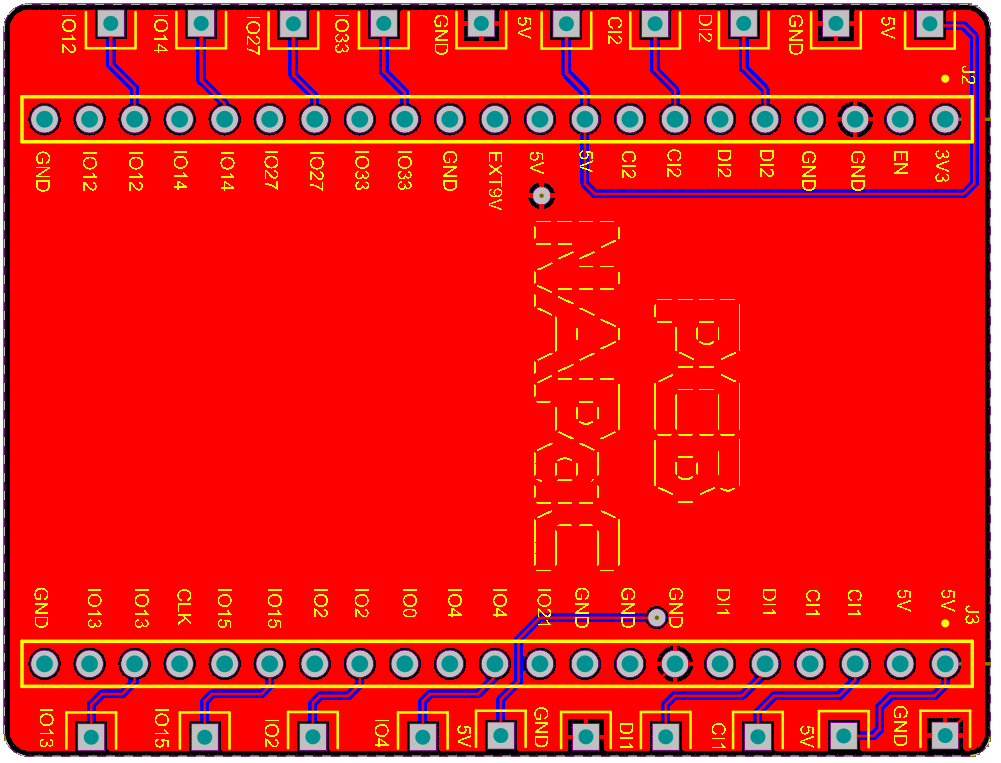
\includegraphics[width=0.6\textwidth]{images/EE_DetachableModule_2D.PNG}
    \caption{Two-dimensional view of the detachable module (realized on \textit{Altium Designer})}
    \label{fig:detachable_module_2D}
\end{figure}

Figure \ref{fig:detachable_module_3D} illustrates the final result of the detachable PCB design.

\begin{figure}[H]
    \centering
    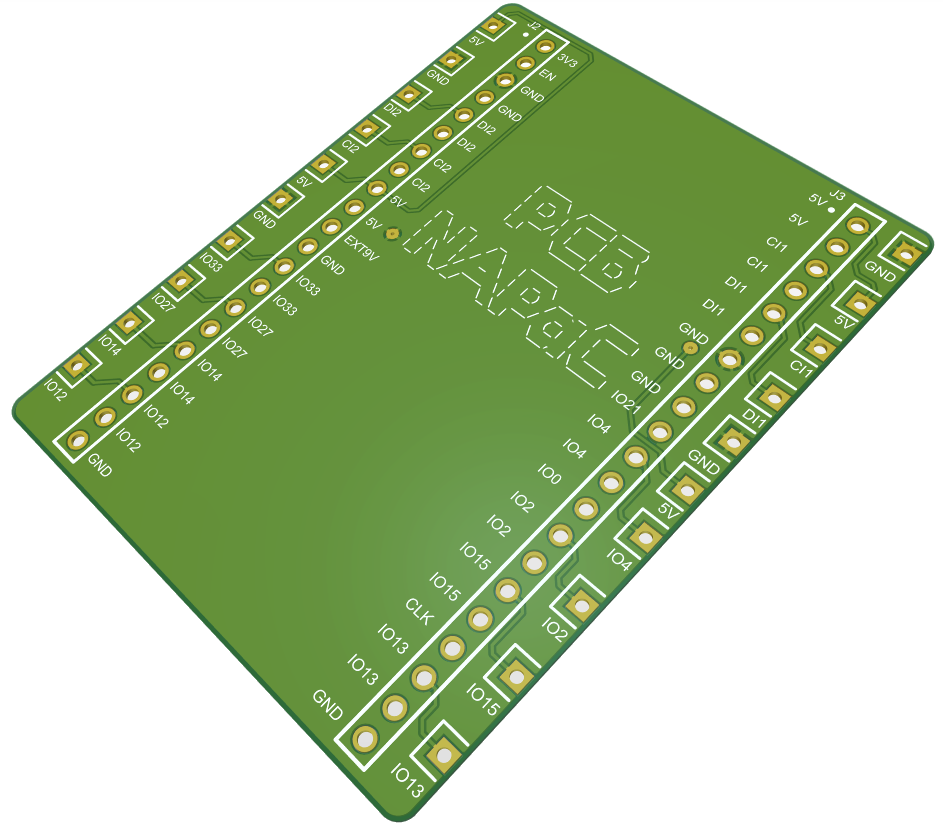
\includegraphics[width=0.6\textwidth]{images/EE_DetachableModule_3D.PNG}
    \caption{Three-dimensional view of the detachable module (realized on \textit{Altium Designer})}
    \label{fig:detachable_module_3D}
\end{figure}

\newpage
\subsection{Next steps for the electronics}
\label{subsec:electronics_next_steps} 

The final aim of our trip to China will be to get at least two fully working prototypes. One plush toy would be kept by Mr. Laperrouza, the founder of the CHIC adventure, who might showcase our prototype to the students of the following CHIC editions. The second plush toy would stay with the \textit{Toygether} team, to eventually present the project to investors or simply keep some good memories from this very rich and interdisciplinary experience. 

\medskip Focusing on the electronic side of the prototype, the aim before landing to China will be to assemble and test the main PCB. The electronics of the plush toy are one of fundamental pieces of this project, that require to be fully functional, in order to get a working prototype. 

\medskip If the prototype results non-functioning after testing it, the goal before the take-off to China will be to spot the problems where the electronics fail, to quickly fix them with a second PCB iteration in China. The main goal of this program is to accelerate this process of testing and getting a functional prototype, by entering into the Chinese electronics fabric of the World.